
  

\chapter{Study of the Existing System}

\section*{Introduction}

This chapter presents a detailed analysis of the existing weather monitoring system in place at Unisphere. The purpose is to understand its current architecture, evaluate its components, and identify its operational strengths and weaknesses. The system includes a combination of sensor hardware, embedded devices, and cloud-based services that together form a pipeline for real-time environmental data acquisition and delivery. Through this analysis, we aim to assess the efficiency, reliability, and scalability of the existing setup, and to highlight opportunities for improvement. These insights provide a foundation for the design and integration of new components in subsequent chapters.

\section{System Description}

\subsection{System Overview}


The system under study is a weather station designed to collect and transmit real-time meteorological data. It integrates a Vaisala WXT536 sensor, which measures parameters such as wind speed, temperature, humidity, pressure, and precipitation. The sensor communicates with a \gls{revpi} industrial controller over an \gls{rs485} interface. On the \gls{revpi}, the data is parsed and formatted before being sent to the cloud via \gls{aws} AppSync. The primary goal of this system is to support Unisphere’s mission of enabling safe and optimized flight operations through the NOVA platform. By providing high-quality, real-time weather data, the system enhances situational awareness, supports trajectory planning, and contributes to safety assessments.\\
Figure~\ref{fig:system-overview-hybrid} illustrates the overall structure of the weather station. 
It highlights the main data flow from the sensors to the RevPi, the cloud, and finally NOVA, while also showing the supporting infrastructure such as power supply, surge protection, and remote management tools.

\begin{figure}[H]
\centering
\begin{adjustbox}{width=\textwidth}
\begin{tikzpicture}[
  font=\small,
  node distance=10mm and 12mm,
  comp/.style={draw, rounded corners=2pt, inner sep=3mm, align=center},
  group/.style={draw, rounded corners=2pt, inner sep=3mm, align=center, fill=black!3},
  flow/.style={-{Latex}, thick},
  mgmt/.style={densely dotted, -{Latex}, thick},
  power/.style={dashed, -{Latex}, thick}
]

% Sensors group
\node[group, label={[label]above:Sensors}] (sensors) 
{\parbox{4.3cm}{\centering \textnormal{\textbf{Vaisala WXT536}\\[-2pt] (ASCII over RS-485, 19200)}}};

% RevPi
\node[comp, right=28mm of sensors] (revpi) 
{\parbox{4cm}{\centering \textnormal{\textbf{RevPi Connect+}\\Raspberry Pi OS (Bookworm)\\Python 3.11 + systemd}}};


% Cloud group
\node[group, right=22mm of revpi, label={[label]above:AWS Cloud}] (cloud) 
{\parbox{5.4cm}{\centering \textnormal{
\textbf{AppSync} (GraphQL API)\\
\textbf{Cognito} (Auth)\\
\textbf{DynamoDB} (Realtime store)\\
\textbf{Lambda / EventBridge / CloudWatch}
}}};

% User apps
\node[comp, right=22mm of cloud] (apps) 
{\parbox{3cm}{\centering \textnormal{\textbf{NOVA}\\Dashboards / APIs}}};

% Power + surge
\node[comp, below=20mm of sensors] (surge) 
{\parbox{3cm}{\centering \textnormal{Vaisala\\Surge Protector}}};
\node[comp, below=18mm of revpi] (psu) 
{\parbox{3.5cm}{\centering \textnormal{DRL-24V480W1EN\\24\,V DC Power Supply}}};

% Management block
\node[comp, above=18mm of revpi] (mgmt) 
{\parbox{3cm}{\centering \textnormal{Qbee / SSH\\(Remote Mgmt)}}};

% Connections
\draw[flow] (sensors.east) -- node[above, sloped]{RS-485 (ASCII)} (revpi.west);
\draw[flow] (revpi) -- node[above, sloped]{Ethernet/4G} (cloud);
\draw[flow] (cloud) -- (apps);

\draw[power] (psu.north) -- ++(0,7mm) -| (revpi.south);
\draw[power] (psu.west) -- ++(-18mm,0) |- (surge.east);
\draw[power] (surge.north) -- ++(0,7mm) -| (sensors.south);

\draw[mgmt] (mgmt) -- (revpi);

% Legend
\node[align=left, anchor=north west] at ($(psu.south west)+(-2mm,-13mm)$) {
\begin{tikzpicture}[x=1cm,y=0.5cm]
\draw[flow] (0,0) -- +(0.8,0) node[right, black]{Data flow};
\draw[power] (0,-0.8) -- +(0.8,0) node[right, black]{Power};
\draw[mgmt] (0,-1.6) -- +(0.8,0) node[right, black]{Remote management};
\end{tikzpicture}
};

\end{tikzpicture}
\end{adjustbox}
\caption{System overview: functional data flow with supporting infrastructure (power, surge, remote management).}
\label{fig:system-overview-hybrid}
\end{figure}




\subsection{Hardware Architecture}

The initial deployment of the weather station system includes a compact yet robust set of components designed for industrial reliability and field deployment. The setup is composed of the Revolution Pi Connect+ as the central processing unit, connected via dedicated RS-485 interfaces to the Vaisala WXT536 and \gls{pwd12} sensors. The \gls{revpi} also connects to the 24 V DC power supply that feeds both sensors. The network connection (Ethernet/4G) provides the link to the cloud backend. This arrangement ensures that each sensor operates on an independent communication bus with the correct baud rate, reducing cross-talk and improving reliability in remote deployments.



%\begin{figure}[H]
%  \centering
%  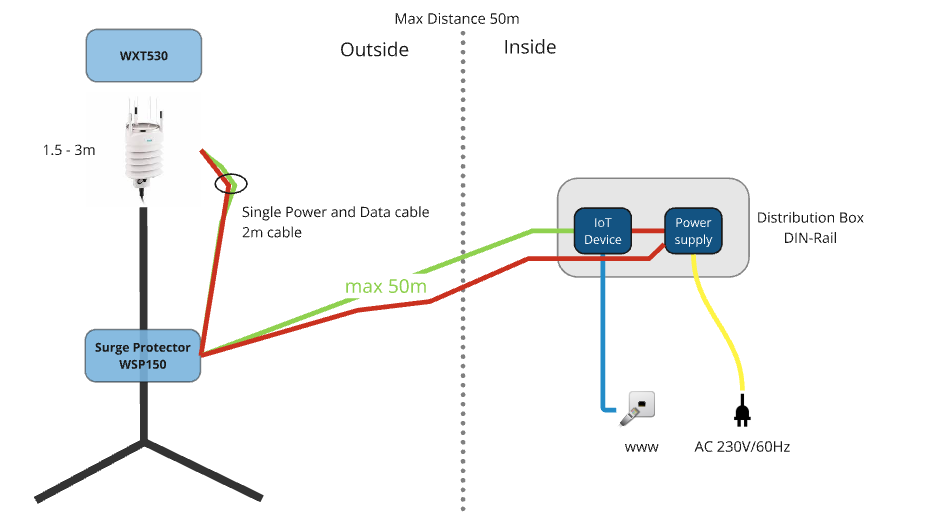
\includegraphics[width=0.8\textwidth]{images/HARD.png}
%  \caption{Actual System Architecture}
%  \label{fig:hard}
%\end{figure}



\subsubsection*{Main Hardware Components}
\begin{itemize}
    \item \textbf{Vaisala WXT536:} Multi-parameter weather sensor measuring wind, temperature, humidity, pressure, and precipitation.
    \item \textbf{\gls{revpi} Connect+:} Industrial Raspberry Pi-based controller responsible for data parsing and cloud integration.
    \item \textbf{DRL-24V480W1EN:} \gls{din}-rail industrial power supply delivering stable 24\,V\,DC.
    \item \textbf{Vaisala Surge Protector:} Protects the system against lightning-induced voltage spikes.
    \item \textbf{Heavy-duty Mast:} A freestanding lamp stand used to mount the sensor outdoors.
    \item \textbf{Industrial Ethernet Switch (IDS-105FE):} Provides network connectivity between \gls{revpi} and backend services.
    \item \textbf{Cables and Connectors:} Including an 8-pin M12 cable for power and \gls{rs485} communication.
\end{itemize}



\subsubsection*{Power and Communication}
\begin{itemize}
    \item \textbf{Power Input:} 230\,V\,AC supplied to the DRL power supply.
    \item \textbf{Sensor Power:} 24\,V\,DC provided to the WXT536.
    \item \textbf{Communication Interface:} RS-485 using an 8-pin M12 connector (differential A/B lines).
    \item \textbf{\gls{revpi} Serial Port:} Typically \texttt{/dev/ttyAMA5} or \texttt{/dev/ttyAMA4} depending on wiring configuration.
\end{itemize}

\subsubsection*{Installation and Protection}
\begin{itemize}
    \item \textbf{Mounting:} Pole-mounted setup suitable for testing and outdoor deployments.
    \item \textbf{Grounding:} Properly grounded and protected against electrical surges.
    \item \textbf{Enclosure:} Components placed in a sealed electrical box for weather protection.
\end{itemize}



\subsection{Communication Interfaces}

The system relies on a combination of serial and cloud-based communication interfaces to ensure seamless data flow from sensor to cloud platform.

\begin{itemize}
  \item \textbf{Sensor-to-Controller Communication:}  
  The Vaisala WXT536 sensor communicates with the \gls{revpi} using the \textbf{\gls{ascii} protocol} over an \textbf{\gls{rs485}} physical interface. The communication is configured at a \textbf{baud rate of 19200}. A twisted pair configuration is used for the \gls{rs485} line, and an M12 8-pin connector is employed to connect the sensor to the electric box.

  \item \textbf{Data Handling on the \gls{revpi}:}  
  Upon reception, the sensor messages are verified using a \textbf{\gls{crc} checksum} to ensure data integrity. Once validated, the data is parsed and formatted into a readable structure for further use and transmission.

  \item \textbf{Controller-to-Cloud Communication:}  
  The parsed weather data is transmitted in real-time to the cloud using \textbf{\gls{aws} AppSync}, a GraphQL-based service that supports low-latency communication. Data is not batched, but pushed directly upon reception and validation.

  \item \textbf{Remote Access and Monitoring:}  
  Remote access to the \gls{revpi} is achieved through \textbf{\gls{ssh}} using its \gls{ip} address when connected to the office Ethernet network. Additionally, \textbf{Qbee} is used as a remote monitoring and management platform, allowing secure access and deployment from external locations.

  \item \textbf{Surge Protection:}  
  Although surge protection is primarily applied to the power lines, the communication setup benefits indirectly from the protected environment within the electric enclosure, reducing the risk of hardware damage.
\end{itemize}


\subsection{Software Stack and Cloud Services}

The system is built around a lightweight but robust software stack running on an industrial-grade controller, with full integration into \gls{aws} cloud services. Figure \ref{fig:cloudflow} presents a high-level view of the software and cloud architecture, illustrating the flow of data from sensor acquisition to real-time cloud transmission and backend interaction. The software and cloud components are structured as follows:


\begin{itemize}
  \item \textbf{Programming Language:}  
  The entire application logic is implemented in \textbf{Python}, which provides a balance between rapid development and system-level hardware communication capabilities.

  \item \textbf{Runtime Environment:}  
  The \gls{revpi} Connect+ controller runs \textbf{Raspbian GNU/Linux 12 (Bookworm)}, a Debian-based operating system. The Python application is executed within a \textbf{\gls{venv}} to ensure package isolation, and is deployed as a \textbf{systemd service} to guarantee automatic startup and resilience after reboots.

  \item \textbf{Data Handling and Parsing:}  
  Sensor data is received via the \gls{rs485} interface and is subject to a \textbf{\gls{crc} checksum validation}. Once validated, the \gls{ascii}-formatted message is parsed into a structured format suitable for cloud transmission. 

  \item \textbf{Cloud Integration:}  
  Real-time weather data is transmitted to the cloud via \textbf{\gls{aws} AppSync}, using a GraphQL \gls{api} endpoint. This allows efficient and structured interaction with backend services while enabling real-time data availability.

  \item \textbf{Authentication and Security:}  
  Authentication is managed via \textbf{\gls{aws} Cognito}, and access to the AppSync endpoint is secured using an \textbf{\gls{api} key}, stored in environment variables to prevent hardcoding credentials within the source code.
  
  \item \textbf{Supporting AWS Services:}  
  In addition to AppSync and Cognito, other AWS services are integrated in the backend to support system monitoring and data processing. These include \textbf{DynamoDB} for storing incoming weather records, \textbf{CloudWatch} for runtime monitoring and logging, and \textbf{EventBridge}, which is used internally for identifying inactive sensors and automating alerting and historical weather data preprocessing.


  \item \textbf{Deployment and Maintenance:}  
  For \gls{vcs}, we use \textbf{Git}. Updates are pushed to the \gls{revpi} either via local access or remotely using \textbf{Qbee}, a device management platform that supports remote monitoring and secure \gls{ssh} access.
\end{itemize}


\begin{figure}[H]
    \centering
    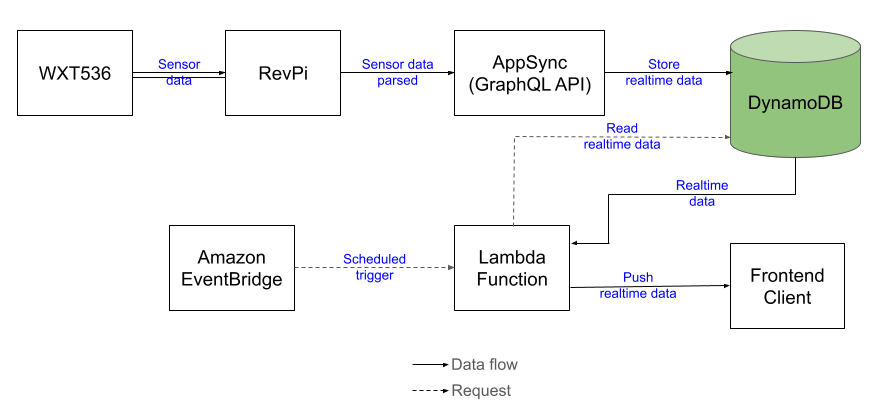
\includegraphics[width=\textwidth]{images/cloud flow.png}
    \caption{Data Flow Architecture}
    \label{fig:cloudflow}
\end{figure}

\section{System Evaluation}

\subsection{System Strengths}

The weather station system designed by Unisphere exhibits several strengths that contribute to its operational effectiveness, maintainability, and integration potential.

\subsubsection{Robustness and Reliability}

The existing system, prior to the integration of the new visibility sensor, was architected for operational stability and reliability in long-term deployments. The software runs as a \texttt{systemd} service on the \gls{revpi}, which ensures automatic restarts in case of unexpected shutdowns or power failures. In addition, error handling mechanisms are implemented through \gls{crc} checksum validation and structured message parsing. These features contribute to reducing the likelihood of system crashes and ensuring consistent data availability over time. 


\subsubsection{Simplicity and Modularity}

The system architecture follows a modular design that separates sensor communication, data parsing, and cloud transmission into distinct functional layers. This separation allows for clear interfaces between components and simplifies both debugging and future extensions. For instance, the code responsible for parsing data from the sensor is encapsulated in independent modules, which can be reused or adapted for other sensors. The availability of an unused RS-485 port on the \gls{revpi} further simplified the physical integration of the new Vaisala \gls{pwd12} sensor, requiring minimal disruption to the existing setup. Overall, the modular structure enables scalable development without requiring a complete system overhaul.


\subsubsection{Cloud Integration}

The system benefits from seamless integration with \textbf{\gls{aws}} cloud services, particularly through the use of AppSync for real-time data streaming. This integration ensures immediate availability of weather data for backend services and frontend applications. AppSync enables efficient communication using GraphQL, which allows clients to fetch precisely the data they need, minimizing payload size and reducing response latency. The use of scalable cloud services also facilitates future extensions, such as long-term storage, alerting, and analytics.

\subsection{Limitations and Opportunities for Improvement}

While the weather station system demonstrates robustness and modularity, certain technical limitations were identified during the integration work. These limitations represent opportunities for further refinement in future system iterations.

\subsubsection{Lack of Visibility Measurement}

The existing weather station provides valuable meteorological data such as wind, precipitation, temperature, humidity, and pressure. However, it does not include visibility measurements, which are critical for aviation-related applications. Visibility data directly supports decision-making for flight safety, landing operations, and trajectory planning. The absence of this parameter reduces the system’s ability to deliver a comprehensive picture of atmospheric conditions.



\subsubsection{Protocol and Communication Constraints}

The system relies on the \gls{rs485} interface for communication with the weather sensors. While \gls{rs485} is reliable for industrial serial communication, it requires all connected devices to operate at the same baud rate. This constraint limits the possibility of using multiple sensors with different serial configurations on the same line.  
Moreover, the current setup uses the \gls{ascii} protocol, which, although simple, is less efficient in terms of message size and validation. Alternative protocols like Modbus \gls{rtu} may offer improvements in reliability and bandwidth usage. A comparative overview is shown in Table~\ref{tab:protocol-comparison}.

\begin{table}[!ht]
\renewcommand{\arraystretch}{1.5}
\centering
\caption{Comparison between \gls{ascii} and Modbus \gls{rtu} protocols}
\label{tab:protocol-comparison}
\begin{tabular}{|c|c|c|}
\hline
\textbf{Aspect} & \textbf{\gls{ascii} Protocol} & \textbf{Modbus \gls{rtu} Protocol} \\
\hline
Message Format & Human-readable characters & Binary format \\
\hline
Bandwidth Efficiency & Lower (larger messages) & Higher (compact messages) \\
\hline
Error Detection & Typically \gls{crc} or checksum & \gls{crc} integrated \\
\hline
Ease of Debugging & Easier (text-based) & Harder (binary) \\
\hline
Message Size & Larger due to encoding & Smaller and more efficient \\
\hline
\end{tabular}
\end{table}

\subsubsection{Lack of Offline Resilience}

The original version of the weather station system was designed with the assumption of continuous internet connectivity. However, operational experience with different customer deployments revealed that connectivity disruptions can occur — for example, due to network outages or infrastructure work within the client’s network environment. In such cases, the system is unable to transmit weather data to the cloud, leading to permanent data loss during the offline period.

This limitation affects the completeness and continuity of the dataset, which are essential for use cases such as real-time monitoring, retrospective analysis, and flight simulation validation. Enhancing the system to support offline buffering and delayed transmission is therefore a critical area for future improvement.

\subsubsection{Data Handling and Storage Gaps}

The current system uses an \textbf{\gls{aws} DynamoDB} table to store incoming weather records, each of which is assigned a \textbf{\gls{ttl}} attribute of 48 hours. This design ensures that outdated entries are automatically deleted, allowing the system to maintain a lightweight and cost-efficient database while supporting real-time weather monitoring.

Although short-term retention is sufficient for most operational needs, certain use cases — such as long-term analysis, retrospective evaluations, or training of predictive models — require permanent access to historical weather data. Figure \ref{fig:cloud improved} illustrates an architectural extension that incorporates a dedicated cloud storage layer. This improvement allows the system to maintain its real-time performance while enabling historical data archiving in a scalable and structured manner.

\begin{figure}[H]
  \centering
  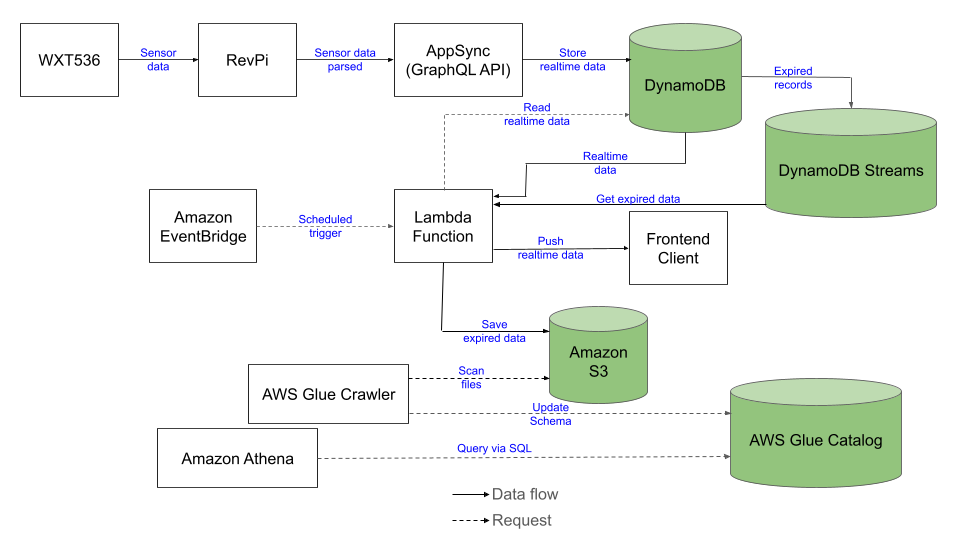
\includegraphics[ width=\textwidth]{images/cloud improved.png}
  \caption{Proposed improvement to cloud architecture with persistent data storage}
  \label{fig:cloud improved}
\end{figure}



\subsubsection{Scope of This Work}

The analysis above highlights three main limitations of the existing weather station system: protocol and communication constraints, gaps in data storage, and lack of offline resilience.  
However, not all of these gaps fall within the scope of the present work.

In this thesis, two aspects are addressed directly:
\begin{itemize}
    \item \textbf{Integration of a new visibility measurement:} The Vaisala PWD12 sensor is added to complement the WXT536 and extend the system’s measurement capabilities.
    \item \textbf{Enhancing offline resilience:} A local buffering mechanism based on SQLite is implemented to prevent data loss during temporary connectivity outages.
\end{itemize}

The following limitations are acknowledged but not solved within this work:
\begin{itemize}
    \item \textbf{Protocol and communication constraints:} A theoretical improvement could be achieved by adopting Modbus RTU instead of ASCII, allowing more efficient message formats and flexible baud rate handling. This would require substantial changes in both firmware configuration and software parsing, and is therefore considered out of scope for this thesis.
    \item \textbf{Data storage gaps:} A potential solution is to introduce a cloud-based persistent storage layer (e.g. Amazon S3 or a time-series database) to complement DynamoDB’s short-term retention. This would enable historical analysis and model training, but lies outside the immediate objectives of this work.
\end{itemize}

This scoping ensures that the thesis remains focused on sensor integration and operational robustness, while still acknowledging other improvement paths for the system.



\section*{Conclusion}
With a clear understanding of the existing weather station system, including its architecture, strengths, and limitations, the focus now shifts to the detailed study of the new visibility sensor selected for integration: the Vaisala \gls{pwd12}. This chapter provided a comprehensive examination of the sensor’s internal design, operating principles, and technical specifications, as well as its relevance to the system’s operational objectives. This foundational understanding is essential to ensure effective hardware integration, data parsing, and long-term reliability within the broader weather monitoring platform.

